\documentclass[12pt]{article}
\usepackage[utf8]{inputenc}
\usepackage{geometry}
\usepackage{svg}
\usepackage{float}
\usepackage{caption}
\usepackage{amsmath,amsthm,amsfonts,amssymb,amscd}
\usepackage{fancyhdr}
\usepackage{titlesec}
\usepackage{hyperref}
\usepackage{listings}
\usepackage[skip=3pt]{parskip}
\usepackage[ngerman]{babel}
\pagestyle{empty}
\titleformat*{\section}{\large\bfseries}
\titleformat*{\subsection}{\bfseries}

%
\geometry{
	a4paper,
	total={170mm,240mm},
	left=20mm,
	top=30mm,
}

\date{}
%Bitte ausfüllen
\newcommand\course{Betriebssysteme}
\newcommand\hwnumber{\large Portfolio 2}
\newcommand\Name{Fabian Sponholz}
\newcommand\Neptun{1561546}

%Matheinheiten
\newcommand\m{\:\textrm{m}}
\newcommand\M{\:\Big[\textrm{m}\Big]}
\newcommand\mm{\:\textrm{mm}}
\newcommand\MM{\:\Big[\textrm{mm}\Big]}
\newcommand\un{\underline}
\newcommand\s{\:\textrm{s}}
\newcommand\bS{\:\Big[\textrm{S}\Big]}
\newcommand\ms{\:\frac{\textrm{m}}{\textrm{s}}}
\newcommand\MS{\:\Big[\frac{\textrm{m}}{\textrm{s}}\Big]}
\newcommand\mss{\:\frac{\textrm{m}}{\textrm{s}^2}}
\newcommand\MSS{\:\Big[\frac{\textrm{m}}{\textrm{s}^2}\Big]}

%Trennlinie
\newcommand\separator{\rule{\linewidth}{0.5pt}}

%Bitte nicht einstellen
\renewcommand{\figurename}{Abbildung}
\renewcommand{\tablename}{Tabelle}
\pagestyle{fancyplain}
\headheight 35pt
\lhead{\Name\\\Neptun}
\chead{\textbf{ \hwnumber}}
\rhead{\course \\ \today}
\lfoot{}
\cfoot{}
\rfoot{\small\thepage}
\headsep 1.5em

\begin{document}
	
\section*{Umgebung der Experimente}
Folgende Tabellen beschreiben das System, auf dem die Tests durchgeführt wurden.
\subsection*{Hardware-Spezifikation}
\begin{table}[h]
	\centering
	\begin{tabular}{|l|l|}
		\hline
		\textbf{Merkmal} & \textbf{Spezifikation} \\
		\hline
		CPU-Bezeichnung & AMD Ryzen 5 4500U with Radeon Graphics\\
		CPU-Architektur & x86 (AMD Renoir) \\
		CPU-Fertigungsverfahren & 7 nm (TSMC) \\
		\hline
		Anzahl Kerne / Threads & 6 / 6 \\
		Basistaktfrequenz & 2.3 GHz \\
		Maximale Boost-Taktfrequenz & 4.0 GHz \\
		\hline
		L1-Cache & 384 KB \\
		L2-Cache & 3 MB \\
		L3-Cache & 8 MB \\
		\hline
		TDP (Thermal Design Power) & 15 Watt \\
		Maximale Temperatur & 105 °C \\
		\hline
		Arbeitsspeicher & 8GB DDR4-3200 \\
		\hline
		Erscheinungsdatum & 07.01.2020 \\
		\hline
	\end{tabular}
\end{table}

\subsection*{Software-Umgebung}
\begin{table}[h]
	\centering
	\begin{tabular}{|l|l|}
		\hline
		\textbf{Merkmal} & \textbf{Spezifikation} \\
		\hline
		Betriebssystem & Arch Linux\\
		Kernel-Version & Linux 6.12.8-arch1-1\\
		\hline
		Java-Version & Java 21\\
		Java-Implementierung & java-21-openjdk\\
		\hline
	\end{tabular}
\end{table}

\section{Aufgabe 1 - Latenz bei Kommunikation mit Spinlock}
\subsection*{Vorgehen zur Latenzmessung}
Bei der Kommunikation über Spinlocks wartet ein Thread auf die Freigabe einer Ressource, indem er fortwährend (z.B. in einer \texttt{while}-Schleife) überprüft, ob die Ressource frei ist. 
Um die Latenz zu messen, habe ich neben dem Main-Thread einen \texttt{Reader}-Thread erstellt, der auf die Freigabe einer Ressource (Boolean, der auf \texttt{true} gesetzt wird) wartet, und den Wert dann wieder auf \texttt{false} setzt. 
Nachdem der Main-Thread den Wert auf \texttt{true} gesetzt hat, wartet er wiederum, bis der Wert wieder auf \texttt{false} gesetzt wird.

Um Race Conditions beim Abfragen der Werte aus den While-Schleifen zu vermeiden, wird der Zugriff mithilfe von \texttt{synchronized} Setter- und Getter-Methoden geregelt.
Jeder Thread trägt immer, wenn er eine Nachricht vom anderen Thread erhält, einen Zeitstempel in Nanosekunden in eine ausreichend große Array-Liste ein, woraus später die Latenz berechnet wird.
Nun folgen Auszüge aus dem Source Code, die dies zeigen.

\begin{lstlisting}[language=java,caption={Latenzmessung im Main Thread}]
for (int i = 0; i < recursions; i++) {
	// set lock to true -> send message
	setLock(true);;
	
	// wait for the return message
	while (getLock()) {
		// Do nothing (spinlock)
	}
	
	// add current time to list
	messageTimes.add(System.nanoTime());
}
\end{lstlisting}

\begin{lstlisting}[language=java,caption={Latenzmessung im Reader Thread}]
while (!isInterrupted()) {
	while (!isInterrupted() && experiment.getLock() == false) {
		// do nothing (spinlock)
	}
	
	// Add the current time to the list
	experiment.getMessageTimes().add(System.nanoTime());
	
	if (isInterrupted()) break;
	
	// Reset the lock (main thread is waiting)
	experiment.setLock(false);
}
\end{lstlisting}


\subsection*{Versuchsaufbau / Implementierung}
Im Ursprünglichen Versuchsaufbau habe ich für jeden Versuchsdurchlauf den \texttt{Reader}-Thread und das \texttt{Experiment}-Objekt neu erstellt und jeweils von jedem Experiment die minimale Latenz gespeichert.
Das Ergebnis des ersten Durchlaufs ist in Abbildung \ref{img:spinlock_first} dargestellt.

Wie man sieht liegt, anders als zu erwarten wäre, keine Normalverteilung der Latenzen vor.
Nach reiflicher Überlegung hatte ich den Verdacht, dass ich durch die Instantiierung einer \texttt{Experiment}- und \texttt{Reader}-Objekts bei jedem Versuch eine große Menge ungenutzter Objekte erzeuge und dadurch ggf. der \emph{Garbage Collector} die Performance zeitweise mindert.

Um einen weiteren Performance-Faktor zu entfernen, habe ich noch die Konstruktion bestehend aus Boolean und synchronized Getter- und Settermethoden gehen einen \emph{AtomicBoolean} ausgetauscht.

Nachdem ich die Implementierung so angepasst habe, dass die bestehenden Objekte in jedem Experiment wiederverwendet werden können, ergab sich tatsächlich eine Normalverteilung der Minima, sodass das 95\%-Konfidenzintervall einfach berechnet werden konnte. Mehr dazu in Abschnitt \ref{sect:results}.

\begin{figure}[H]
	\centering
	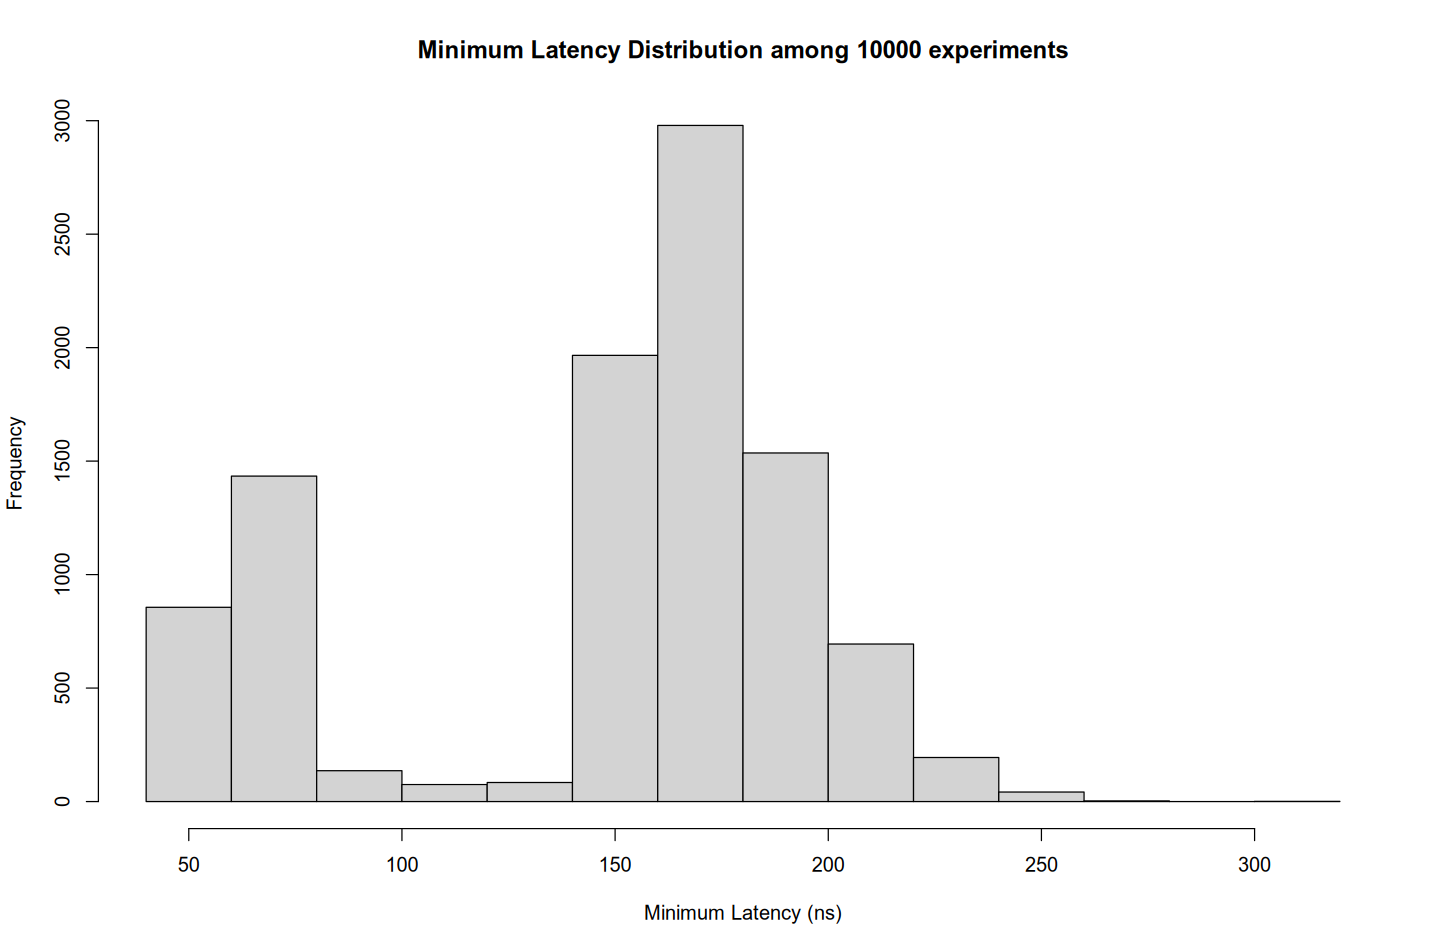
\includegraphics[width=0.75\textwidth]{./img/spinlock_first_try}
	\caption{Verteilung der Minima im ersten Experiment}
	\label{img:spinlock_first}
\end{figure}


\section{Ergebnisse}
\label{sect:results}

\subsection*{Aufgabe 1 - Spinlock}
Es wurden 1000 Durchläufe des Experiments durchgeführt mit jeweils 50000 Wiederholungen der Messung, wobei jeweils zwei Latenzen gemessen wurden (Hin- und Rückweg).
Insgesamt wurden pro Experiment also 100000 Latenzen gemessen und jeweils das Minimum gespeichert.
Hier die Ergebnisse:
\begin{figure}[H]
	\centering
	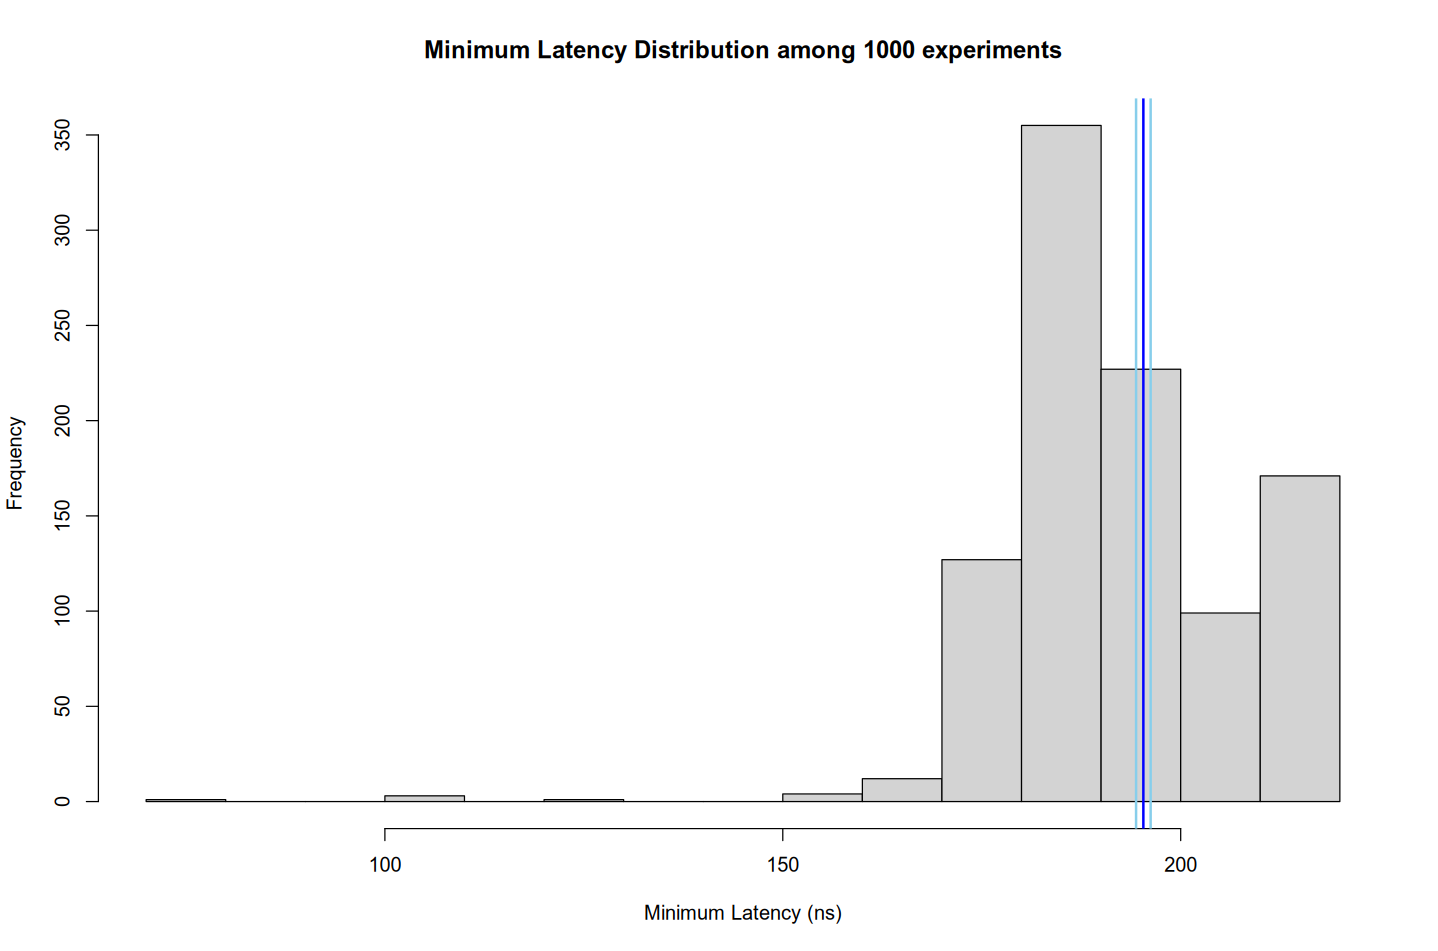
\includegraphics[width=0.75\textwidth]{./img/spinlock_second}
	\caption{Verteilung der Minima mit 95\%-Konfidenzintervall (blau)}
	\label{img:spinlock_second}
\end{figure}

\begin{itemize}
	\item Durchschnittliche minimale Latenz: $182,89 ns$
	\item 95\%-Konfidenzintervall: $182,45 ns - 183,34 ns$
\end{itemize}

Die Verteilung weist dabei eine  deutliche Linksschiefe und einen Bruch beim Maximum von $210 ns$ auf.


\end{document}